\documentclass{IEEEtran}

%% Additional Packages
\usepackage{cite}
\usepackage{graphicx}
\usepackage{algorithm}
\usepackage{algpseudocode}
\usepackage{siunitx}
\usepackage[utf8]{inputenc}

%% Macros
\newcommand{\mb}[1]{\mathbf{#1}}
\renewcommand\IEEEkeywordsname{Keywords}

\title{FPGA Implementation of a LSTM Neural Network}

%% COMMENT THIS FOR SUBMISSION
\author{
\IEEEauthorblockN{José Fonseca\IEEEauthorrefmark{1}, João Canas Ferreira\IEEEauthorrefmark{1}, Ivo Timóteo\IEEEauthorrefmark{2}}\\
\IEEEauthorblockA{FEUP\IEEEauthorrefmark{1}, University of Cambridge\IEEEauthorrefmark{2}}
}
%%\IEEEspecialpapernotice{(Working Version)}


\begin{document}

\maketitle

\begin{abstract}
Our work proposes a hardware architecture for a Long Short-Term Memory (LSTM) Neural Network, aiming
to outperform software implementations, by exploiting its inherent parallelism.
The main design decisions are presented, along with the proposed network architecture. A description of the main
building blocks of the network is also presented. The network is synthesized for various sizes and platforms,
and the performance results are presented and analyzed. Our synthesized network achieves a 251 times speed-up
over a custom-built software network, running on a Desktop computer, and a 14 times speed up over the current state of the art.
\end{abstract}

\begin{IEEEkeywords}
Neural Networks, Long Short-Term, FPGA, Reconfigurable Hardware, Machine Learning
\end{IEEEkeywords}

\section{Introduction}\label{sec:intro}
\IEEEPARstart{N}{eural} Networks are one of the most commonly used techniques in Deep Learning. This
particular type of network, a Long Short-Term Memory (LSTM) Network, is a recursive neural network, with memory.
These algorithms have been profusely implemented in software, and their practical applications are plentiful.
However, the benefits of the inherent parallelism offered by a dedicated hardware
platform are not exploited, and there are relatively few implementations of Machine Learning algorithms in
these kind of platforms.

\section{LSTM Neural Networks}\label{sec:lstmnn}
LSTM Networks were originally formulated in~\cite{Hoch97}, and their operation is detailed in Equations~\ref{eq:equationsLSTM}.

\begin{eqnarray}
    \mb{z}^{(t)} & = & g(\mb{W}_z \mb{x}^{(t)} + \mb{R}_z \mb{y}^{(t-1)} + \mb{b}_z) \nonumber\\
    \mb{i}^{(t)} & = & \sigma(\mb{W}_i \mb{x}^{(t)} + \mb{R}_i \mb{y}^{(t-1)} + \mb{p}_i \odot \mb{c}^{(t-1)} + \mb{b}_i) \nonumber\\
    \mb{f}^{(t)} & = & \sigma(\mb{W}_f \mb{x}^{(t)} + \mb{R}_f \mb{y}^{(t-1)} + \mb{p}_f \odot \mb{c}^{(t-1)} + \mb{b}_f) \nonumber\\
    \mb{o}^{(t)} & = & \sigma(\mb{W}_o \mb{x}^{(t)} + \mb{R}_o \mb{y}^{(t-1)} + \mb{p}_o \odot \mb{c}^{(t)} + \mb{b}_o) \nonumber\\
    \mb{c}^{(t)} & = & \mb{i}^{(t)} \odot \mb{z}^{(t)} + \mb{f}^{(t)} \odot \mb{c}^{(t-1)} \nonumber \\
    \mb{y}^{(t)} & = & \mb{o}^{(t)} \odot h(\mb{z}^{(t)}) \label{eq:equationsLSTM},
\end{eqnarray}
where $\odot$ is the Hadamard multiplication. A layer has $N$ LSTM neurons and $M$ inputs (i.e. the size of the layer that
precedes this).

Hitherto, there is but one actual implementation of an LSTM network in hardware, published recently
(March 2016) by Chang et al.~\cite{Chang15}.

\section{Proposed Architecture}\label{sec:proparch}

\subsection{Network Architecture}\label{sec:proprarch_net}
Equations~\ref{eq:equationsLSTM} suggest that the signals $\mb{z}^{(t)}$, $\mb{i}^{(t)}$, $\mb{f}^{(t)}$ and $\mb{o}^{(t)}$ do not depend on each other -- they
operate only on the current input vector $\mb{x}^{(t)}$ and the previous layer output $\mb{y}^{(t-1)}$ -- and therefore can be calculated in parallel. Furthermore, we
can avoid a naive translation of the Equations~\ref{eq:equationsLSTM}, which would replicate unnecessary resources (such as elementwise multipliers
and activation function calculators) and require more area to save a negligible number of clock cycles, by noting that one of the operands is the output
of a $\tanh(\mb{x})$ block and the other of a $\sigma(\mb{x})$, and they are then multiplied (elementwise, of course) together. Instead of replicating
these `$\tanh$-$\sigma$-$(\cdot)$wise' structures, we use a \emph{single one} and choose the operand according to the state that the network is currently in. The
issue about the elementwise multiplier for $\mb{c}^{(t)}$, which does not use the $\tanh$ activation function, can be solved by adding another multiplexer that chooses
between the output of the $\tanh(\mb{x})$ module or the signal $\mb{c}^{(t-1)}$.

The total requirement for DSP slices is
\begin{equation}\label{eq:numdsp_network-opt}
    4\frac{2N}{K_G} + 2N + N = N \left( \frac{8}{K_G} + 3 \right).
\end{equation}

On the other hand, the number of clock cycles needed to output a result is simply
\begin{equation}\label{eq:numcc_network-opt}
    (N \cdot K_G + 6) + 27  = 33 + N\cdot K_G.
\end{equation}

\section{Results}\label{sec:results}
\subsection{Validation}\label{sec:res-val}

The functionality of the network was verified against a Python model of an LSTM network that was developed as a reference,
both for the forward propagation of the network, as well as for the training algorithm.

The learning problem presented to both the software and hardware network is the \textbf{addition} of two binary numbers of 8 bits. The $i$-th
bit of each number is fed to the network as a vector, and the network outputs its prediction of the correct value of the $i$-th bit
of the \emph{result}. After the whole number is processed, the memory cells of the LSTM network are reset and a new addition
task can be presented to the network.

\subsection{Synthesis}\label{sec:results_synth}
The proposed network was first synthesized for a Xilinx XC7Z020 SoC, for sizes $N \in \left\{4, 8, 16, 32\right\}$, varying the resource sharing parameter $K_G$, while keeping $M=2$.
For a network size of 32 and $K_G=8$, the LUT usage exceeded the LUT resources available in the FPGA, so only lower values of $K_G$ were
successfully synthesized. To synthesize the design for sizes $N \in \left\{64, 128 \right\}$ a Virtex-7 VC707 board was used, which has a XC7VX485T (speed grade -2) FPGA core.

\subsubsection{Maximum Frequency}\label{sec:results_synth_maxfreq}
For $N=4$, since there are only 4 rows to be multiplied, the maximum value of $K_G$ is 4, and hence no synthesis was performed for $K_G = 8$ (N.A.); also,
since $K_G = 2$ and $N=32$, it would use $32(8/2+3) = 224$ DSP slices, and that exceeds the 220 slices
available in the XC7Z020, so there is no synthesis data (N.D.), as well.

Increasing $K_G$, the maximum clock speed decreases, and that decrease is steeper for larger values
of $K_G$. This means that there is a critical path in the Matrix-Vector multiplication unit, whose multiplexer becomes
increasingly complex. On the other hand, when $K_G$ is the same, smaller networks are faster
than larger networks. The fastest design is an $N=4$ and $K_G = 2$ network, with a clock frequency of $158.228$ MHz, and
the slowest one is an $N=32$ and $K_G=4$ network, clocked at $101.523$ MHz. The reference design used for validation in
Section~\ref{sec:res-val} is an $N=8$ and $K_G=2$ network clocked at $154.321$ MHz, which yields a clock period of
\SI{6.48}{\nano\second}. The maximum clock frequency for the VC707 was 140.854 MHz for both $N=64$ and $N=128$.


\subsection{Performance}
To evaluate the throughput of the system, a metric was defined based on how many predictions it can produce per second (i.e. produce a new result bit in the output sequence),
in \textbf{millions}. Hence, we multiply the number of clock cycles yielded by Equation~\ref{eq:numcc_network-opt} by the equivalent clock period
from the synthesis clock report for each network. The Python code was run on an i7-3770k Intel Processor, running at 4.2GHz, with 8GB of RAM.

\begin{table}
	\caption{Total processing time for a single forward propagation on the XC7Z020}
	\label{tab:process-time}
    \centering
    \begin{tabular}{ | l | c | c | c | c | c | }
    \hline
    & $K_G=8$  & $K_G=4$ & $K_G=2$ & Python & Speed-up \\
    \hline
    $N=4$ & N.A.  & 309.68 ns  & 259.12 ns & 65 $\mu$s & $\times251$ \\
    \hline
    $N=8$ & 793.46 ns  & 421.12 ns  &  317.52 ns & 72 $\mu$s & $\times228$ \\
    \hline
    $N=16$ & 1.497 $\mu$s  & 738.19 ns  & 461.336 ns & 96 $\mu$s & $\times208$ \\
    \hline
    $N=32$ & N.D.          & 1.586 $\mu$s & N.A.       & 185 $\mu$s  &  $\times117$ \\
		\hline
  \end{tabular}
\end{table}
The hardware network is, at best, $\times251$ faster than the software counterpart,
and at worst $\times117$ faster.
Inverting the values in Table~\ref{tab:process-time}, we know how many forward propagations the network can produce, per second. These values are presented in Figure~\ref{fig:Mclass-psec}.
While the $N=8$ and $K_G=2$ network is able to perform around 3.15 million predictions per second, the Python model can only output around 14 thousand predictions.

\begin{figure}
    \centering
    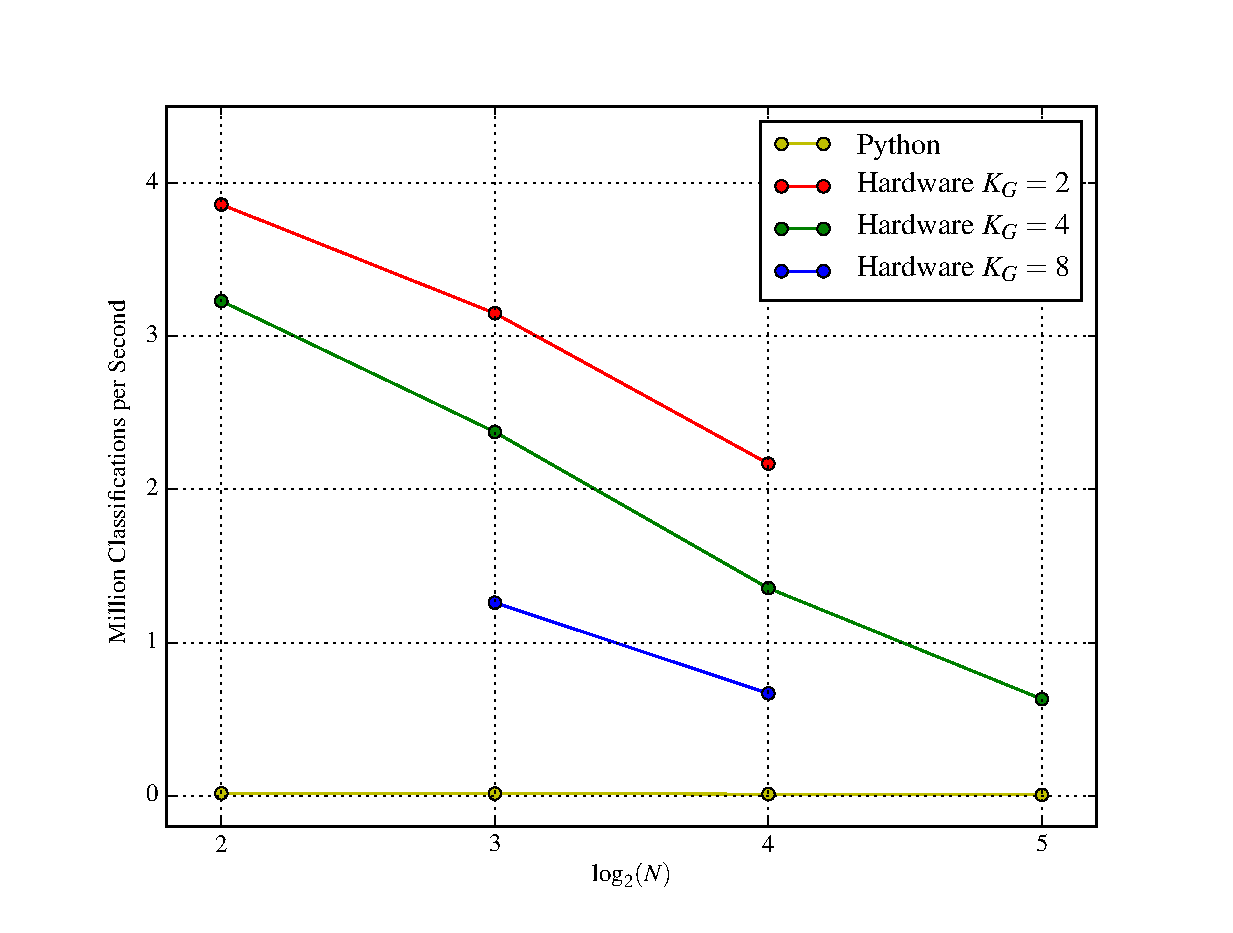
\includegraphics[width=\linewidth]{figures/Mclass-psec.eps}
    \caption[Millions of classifications per second of each design according to the network size $N$]{Millions of classifications per second of each design according to the network size $N$. The comparison is between the software Python model and 3 networks of different levels of resource sharing $K_G$.}
    \label{fig:Mclass-psec}
\end{figure}

As for the larger-sized networks synthesized in the VC707, the results are also very promising. For network sizes of $N=64$ and $N=128$, a complete
forward propagation takes 1.14 $\mu$s and 2.052 $\mu$s respectively, and for both the maximum clock frequency achievable was 140.845 MHz. Since the
design~\cite{Chang15}, for $N=128$, takes an estimated \SI{29.13}{\micro\second}, our design yields an improvement of $14\times$
over it.
%In terms of millions of operations per second (Mops), for an $N=128$ network as the one of~\cite{Chang15}, our work achieves \num{4534.8} Mops per second
%while theirs only achieves \num{264.4} Mops per second. This is because, as stated in~\cite{Chang15}, a network of this size performs \num{132.1d3} Mops, and since
%our work outputs a sample every $1 \over \SI{29.13}{\micro\second}$, we have that 4534.8 Mops per sec. $=\frac{\num{132.1d3} \; \text{Mops}}{\SI{29.13}{\micro\second}}$.

\section{Conclusion}\label{sec:concl}
The LSTM Hardware architecture presented surpassed the performance of the custom-built software implementation by $251\times$, at best,
and also the only current hardware implementation by $14\times$, and solely making use of internal FPGA
resources, achieving a higher level of parallelism. The higher levels of parallelism of this work are achieved at the cost of increasing
design complexity, which limits its scalability to higher sized networks, unlike the implementation of Chang et al.~\cite{Chang15}.
On the other hand, the HDL description of this work is parameterized, and is thus very flexible for networks of any size, not requiring
a redesign of the system every time a differently sized network is required. Furthermore, making use of internal memory makes it suitable
for including an on-chip learning system that can perform training on the network weights.

Given these results, this architecture advances the current state of the art in LSTM Neural Networks
hardware implementations, providing the most efficient implementation to date.

\bibliographystyle{IEEEtran}
\bibliography{bibliography}

\end{document}
